\documentclass{article} % For LaTeX2e
\usepackage[preprint]{colm2026_conference}

\usepackage{microtype}
\usepackage{hyperref}
\usepackage{url}
\usepackage{booktabs}
\usepackage{graphicx}
\usepackage{amsmath}
\usepackage{amssymb}
\usepackage{natbib}

\definecolor{darkblue}{rgb}{0, 0, 0.5}
\hypersetup{colorlinks=true, citecolor=darkblue, linkcolor=darkblue, urlcolor=darkblue}

\title{Stable Reasoning, Fragile Answers: How LLMs Fail at the Final Execution Step Under Semantic Variation}

\author{Arut Selvan Dhanasekaran \\
Independent Researcher \\
\texttt{arutselvan710@gmail.com}
}

\newcommand{\fix}{\marginpar{FIX}}
\newcommand{\new}{\marginpar{NEW}}

\begin{document}

\maketitle

\begin{abstract}
Large language models (LLMs) exhibit significant improvements in complex problem-solving when prompted to generate step-by-step reasoning chains. However, the faithfulness of these reasoning chains---whether they genuinely cause the final answer or merely serve as post-hoc rationalizations---remains a subject of intense debate. In this paper, we introduce the Answer-Reasoning Consistency Gap (ARCG), a novel metric that quantifies the decoupling between reasoning stability and answer stability under natural semantic variation. We evaluate five open-source LLMs (Llama 3.1 8B, Qwen 2.5 14B, Mistral 7B, Gemma 2 9B, and Phi-4 14B) across mathematical and logical reasoning benchmarks using systematic paraphrasing. Contrary to the post-hoc rationalization hypothesis, which predicts stable answers supported by varying rationalizations, we find that ARCG is universally negative across all tested models. Specifically, reasoning chains remain highly consistent across paraphrases, while the final answers derived from those chains exhibit significant fragility. This finding suggests that LLMs learn robust, template-like reasoning patterns but frequently fail at the final logical execution step when the surface-level wording of the prompt changes. We discuss the implications of this ``execution gap'' for the reliability and interpretability of chain-of-thought reasoning.
\end{abstract}

\section{Introduction}

The introduction of Chain-of-Thought (CoT) prompting \citep{wei2023chainofthoughtpromptingelicitsreasoning, kojima2023largelanguagemodelszeroshot} has fundamentally transformed the capabilities of large language models (LLMs) on complex reasoning tasks. By generating intermediate reasoning steps before producing a final answer, LLMs achieve state-of-the-art performance on mathematical, logical, and commonsense benchmarks \citep{cobbe2021training, hendrycks2021measuring}. However, the success of CoT has raised a critical interpretability question: are these generated reasoning chains faithful explanations of the model's internal decision-making process, or are they merely post-hoc rationalizations that mimic human-like logic without causally determining the output?

Recent work has cast doubt on the faithfulness of CoT reasoning. \citet{turpin2023languagemodelsdontsay} demonstrated that LLMs often generate plausible reasoning chains that contradict their actual reliance on biased context. Similarly, \citet{lanham2023measuringfaithfulnesschainofthoughtreasoning} showed that models frequently arrive at the correct answer even when their reasoning chains are artificially truncated or corrupted. Furthermore, \citet{Jiang2025RobustAF} introduced the ``decoupling hypothesis,'' demonstrating through adversarial gradient attacks that an LLM's reasoning can be completely collapsed while its final answer remains robust. These findings collectively suggest that LLMs may decide on an answer early in the generation process and subsequently construct a rationalization to support it.

In this paper, we investigate the faithfulness of CoT reasoning from a different angle: natural semantic variation. Rather than employing adversarial attacks or biased contexts, we ask a simpler question: how does an LLM's reasoning and final answer change when the exact same problem is phrased in slightly different ways? If CoT is primarily post-hoc rationalization, we would expect the model to consistently arrive at the same final answer across paraphrases, while generating varying reasoning chains to justify it. Conversely, if the reasoning chain is a rigid template, we might expect the reasoning to remain stable while the final answer fluctuates.

To formalize this inquiry, we introduce the Answer-Reasoning Consistency Gap (ARCG). ARCG measures the difference between Final Answer Consistency (FAC)---the frequency with which a model produces the same answer across paraphrases---and Reasoning Step Consistency (RSC)---the semantic similarity of the generated reasoning chains. We evaluate five state-of-the-art open-source LLMs on a curated benchmark of mathematical and logical reasoning tasks, generating five systematic paraphrases per problem.

Our results reveal a surprising and universal phenomenon: ARCG is consistently negative across all models. The semantic similarity of the reasoning chains (RSC) is significantly higher than the consistency of the final answers (FAC). This indicates that LLMs apply highly stable, template-like reasoning patterns regardless of how a question is phrased, but frequently fail to execute the final logical step correctly, leading to divergent answers. We term this phenomenon the ``execution gap.'' This finding challenges the prevailing post-hoc rationalization narrative and suggests that the fragility of LLM reasoning lies not in the generation of the logical steps, but in the brittle execution of those steps into a concrete conclusion under semantic variation.

\section{Related Work}

\textbf{Chain-of-Thought Prompting and Faithfulness.} The efficacy of CoT prompting is well-documented \citep{wei2023chainofthoughtpromptingelicitsreasoning, kojima2023largelanguagemodelszeroshot, zhou2023leasttomostpromptingenablescomplex}. However, the faithfulness of these explanations---whether they accurately reflect the model's true reasoning process---is a major concern \citep{jacovi2020faithfullyinterpretablenlpsystems}. \citet{turpin2023languagemodelsdontsay} showed that LLMs can generate unfaithful CoT explanations when influenced by user sycophancy or biased contexts. \citet{lyu2023faithfulchainofthoughtreasoning} attempted to enforce faithfulness by translating natural language reasoning into symbolic programs. Our work differs by evaluating faithfulness through the lens of consistency under natural semantic variation, rather than through adversarial or symbolic interventions.

\textbf{Reasoning Consistency and Robustness.} The robustness of LLMs to prompt variations is a known challenge \citep{webson-pavlick-2022-prompt, jiang2020knowlanguagemodelsknow}. Techniques like Self-Consistency \citep{wang2023selfconsistencyimproveschainthought} and Self-Para-Consistency \citep{chen-etal-2024-self-para} leverage this variability by sampling multiple reasoning paths or paraphrases and applying majority voting to improve accuracy. However, these methods treat reasoning variability as a feature to be exploited rather than a phenomenon to be analyzed. \citet{Ju2025ReasoningPD} measured reasoning path divergence to curate better training data, but did not contrast it with answer consistency. Our ARCG metric explicitly quantifies the gap between reasoning stability and answer stability.

\textbf{The Decoupling Hypothesis.} The work most closely related to ours is \citet{Jiang2025RobustAF}, which proposed the decoupling hypothesis. They demonstrated that adversarial gradient attacks can destroy an LLM's reasoning chain without altering its final answer, suggesting that answers and reasoning are generated independently. While their findings support the post-hoc rationalization theory under adversarial conditions, our experiments using natural paraphrases reveal the opposite effect: reasoning is highly stable, but answers are fragile. This highlights a critical distinction between adversarial vulnerability and natural semantic robustness in LLM reasoning.

\section{Methodology}

\subsection{The Answer-Reasoning Consistency Gap (ARCG)}

To quantify the decoupling between reasoning and answers, we define three metrics evaluated over a set of $N$ semantically equivalent paraphrases of a single problem.

\textbf{Final Answer Consistency (FAC).} FAC measures the proportion of paraphrase pairs that yield the identical final answer. Let $A = \{a_1, a_2, \dots, a_N\}$ be the set of extracted final answers for the $N$ paraphrases. FAC is defined as:
\begin{equation}
\text{FAC} = \frac{2}{N(N-1)} \sum_{i=1}^{N-1} \sum_{j=i+1}^{N} \mathbb{I}(a_i = a_j)
\end{equation}
where $\mathbb{I}$ is the indicator function. FAC ranges from 0 (all answers different) to 1 (all answers identical).

\textbf{Reasoning Step Consistency (RSC).} RSC measures the semantic similarity of the reasoning chains generated before the final answer. Let $R = \{r_1, r_2, \dots, r_N\}$ be the set of reasoning chains (with the final answer stripped). We embed each chain using a pre-trained sentence transformer \citep{reimers-gurevych-2019-sentence} to obtain dense vectors $\mathbf{v}_i$. RSC is the average pairwise cosine similarity:
\begin{equation}
\text{RSC} = \frac{2}{N(N-1)} \sum_{i=1}^{N-1} \sum_{j=i+1}^{N} \cos(\mathbf{v}_i, \mathbf{v}_j)
\end{equation}
RSC ranges from -1 to 1, though in practice it is bounded between 0 and 1.

\textbf{Answer-Reasoning Consistency Gap (ARCG).} The ARCG is simply the difference between FAC and RSC:
\begin{equation}
\text{ARCG} = \text{FAC} - \text{RSC}
\end{equation}
A positive ARCG indicates that the model converges on the same answer more reliably than it produces consistent reasoning (supporting post-hoc rationalization). A negative ARCG indicates that the reasoning is more stable than the final answer (supporting execution fragility).

\subsection{Experimental Setup}

\textbf{Benchmark Dataset.} We curated a benchmark of 30 problems, evenly split between mathematical reasoning (15 problems from GSM8K \citep{cobbe2021training}) and logical reasoning (15 problems from the AI2 ARC-Challenge \citep{clark2018think}). The problems were stratified by difficulty (Easy, Medium, Hard) based on their original dataset annotations.

\textbf{Paraphrase Generation.} For each of the 30 base problems, we generated 5 systematic paraphrases using a strong LLM (Llama 3.1 8B), resulting in 6 total variations per problem (the original plus 5 paraphrases). The paraphrasing strategies were designed to alter the surface-level syntax without changing the underlying semantics or numerical values. The strategies included: formal restatement, informal restatement, passive voice restructuring, step-by-step decomposition, and analogical reformulation. This yielded a total of 180 unique prompts.

\textbf{Models Evaluated.} We evaluated five state-of-the-art open-source LLMs that fit within a 16GB VRAM constraint (RTX 4080): Llama 3.1 8B \citep{touvron2023llama}, Qwen 2.5 14B \citep{bai2023qwentechnicalreport}, Mistral 7B v0.3 \citep{jiang2023mistral7b}, Gemma 2 9B \citep{gemma2024}, and Phi-4 14B \citep{abdin2024phi3}. All models were run locally using the Ollama framework with greedy decoding (temperature = 0.0) to isolate the effects of semantic variation from sampling variance.

\textbf{Inference and Extraction.} Each model was prompted with the 180 variations using a standard zero-shot CoT prompt (``Let's think step by step''). The responses were parsed using regular expressions to separate the reasoning chain from the final answer. For RSC computation, we utilized the \texttt{all-MiniLM-L6-v2} sentence transformer model.

\section{Results}

\subsection{The Universal Negative Gap}

The central finding of our experiments is that ARCG is universally negative across all five evaluated models. As shown in Table \ref{tab:main_results} and Figure \ref{fig:fac_rsc}, Reasoning Step Consistency (RSC) consistently outpaces Final Answer Consistency (FAC). 

\begin{table}[h]
\centering
\caption{Average FAC, RSC, and ARCG across all 30 problems for the five evaluated models. All models exhibit a strongly negative ARCG, indicating that reasoning chains are significantly more stable than final answers across semantic paraphrases.}
\label{tab:main_results}
\begin{tabular}{lcccc}
\toprule
\textbf{Model} & \textbf{Accuracy} & \textbf{FAC} & \textbf{RSC} & \textbf{ARCG} \\
\midrule
Llama 3.1 8B & 0.633 & 0.482 & 0.774 & \textbf{-0.292} \\
Qwen 2.5 14B & 0.583 & 0.353 & 0.801 & \textbf{-0.447} \\
Mistral 7B & 0.383 & 0.193 & 0.751 & \textbf{-0.558} \\
Gemma 2 9B & 0.567 & 0.431 & 0.791 & \textbf{-0.360} \\
Phi-4 14B & 0.617 & 0.400 & 0.808 & \textbf{-0.408} \\
\bottomrule
\end{tabular}
\end{table}

\begin{figure}[h]
\centering
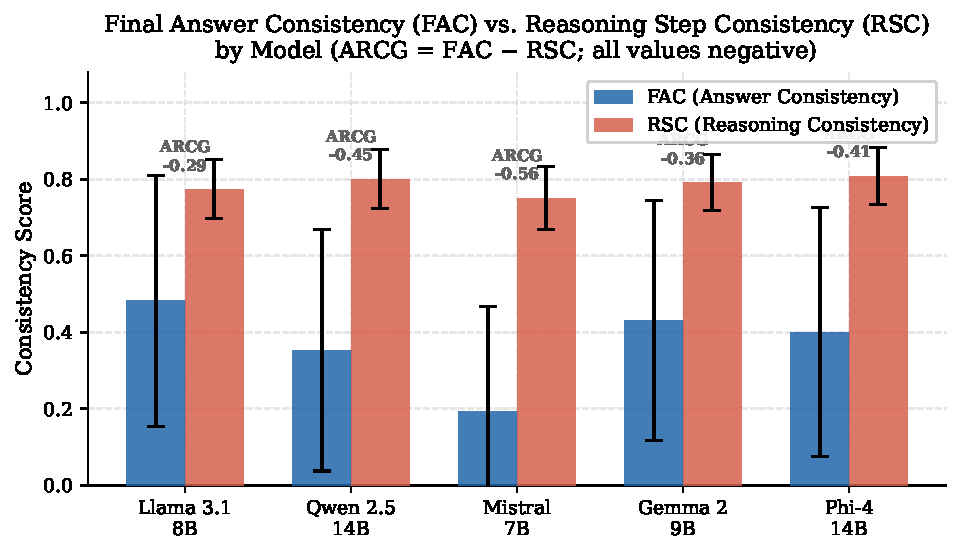
\includegraphics[width=0.8\linewidth]{../figures/fig1_fac_rsc.pdf}
\caption{Comparison of Final Answer Consistency (FAC) and Reasoning Step Consistency (RSC) across models. The gap between the two bars represents the ARCG, which is consistently negative.}
\label{fig:fac_rsc}
\end{figure}

This result directly contradicts the expectation of post-hoc rationalization under natural semantic variation. If models were deciding on an answer first and rationalizing later, we would expect high FAC and lower RSC. Instead, the high RSC scores (ranging from 0.751 to 0.808) indicate that the models are retrieving and applying highly stable, template-like reasoning structures regardless of how the prompt is phrased. However, the low FAC scores (ranging from 0.193 to 0.482) demonstrate that the models frequently fail to execute these stable reasoning templates into a consistent final answer.

\subsection{Domain and Difficulty Effects}

We further analyzed the ARCG across different problem domains and difficulty levels. Figure \ref{fig:domain_difficulty} illustrates these breakdowns.

\begin{figure}[h]
\centering
\begin{minipage}{0.48\textwidth}
  \centering
  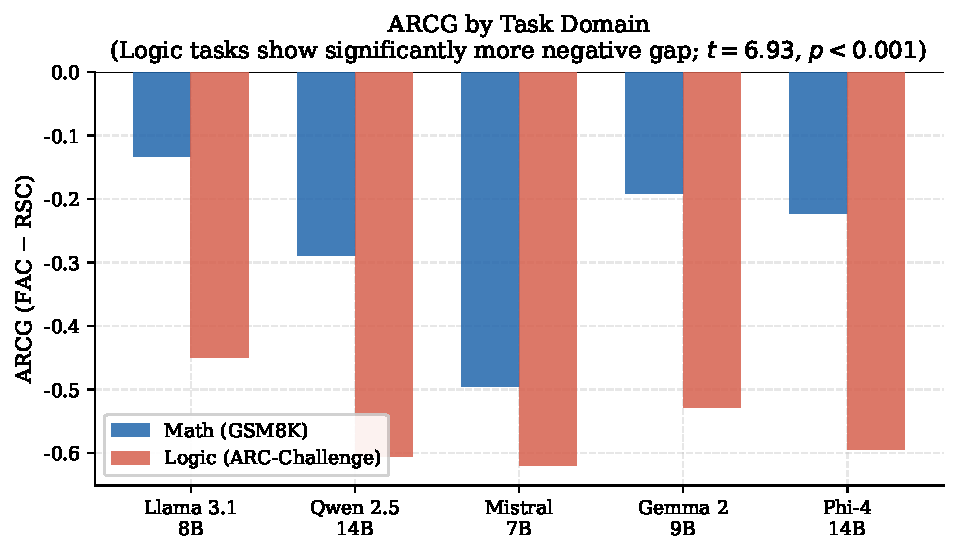
\includegraphics[width=\linewidth]{../figures/fig2_arcg_domain.pdf}
\end{minipage}\hfill
\begin{minipage}{0.48\textwidth}
  \centering
  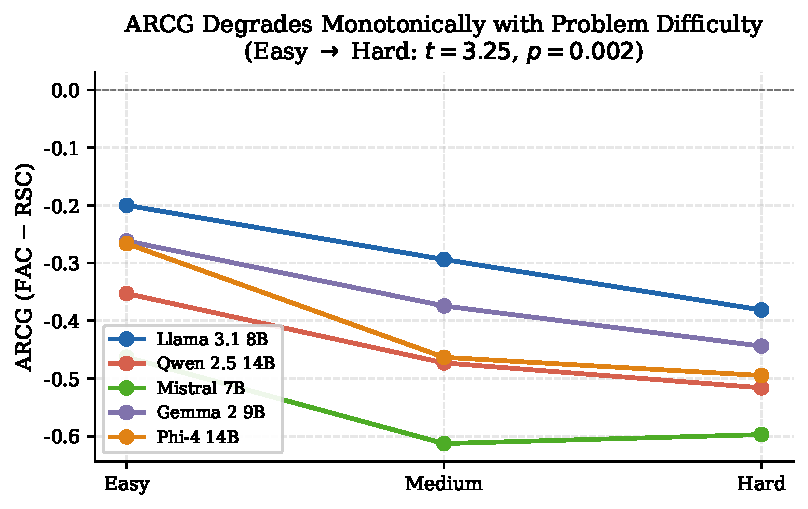
\includegraphics[width=\linewidth]{../figures/fig3_arcg_difficulty.pdf}
\end{minipage}
\caption{Left: ARCG by problem domain. Logical reasoning tasks exhibit a significantly wider (more negative) gap than mathematical tasks. Right: ARCG by problem difficulty. The gap widens monotonically as problem difficulty increases.}
\label{fig:domain_difficulty}
\end{figure}

\textbf{Domain Differences.} The negative ARCG is significantly more pronounced in logical reasoning tasks (ARC-Challenge) compared to mathematical tasks (GSM8K). While mathematical reasoning often involves rigid algorithmic steps that constrain the final answer, logical reasoning requires more nuanced semantic interpretation. The wider gap in logic tasks suggests that while the models can retrieve the correct logical framework (high RSC), the final deduction step is highly sensitive to the specific wording of the premises.

\textbf{Difficulty Degradation.} We observed a monotonic widening of the ARCG as problem difficulty increases. For easy problems, FAC is relatively high, keeping the gap narrow. As difficulty increases, RSC remains remarkably stable---the models still attempt to apply the same reasoning templates---but FAC collapses, leading to a severely negative ARCG. This reinforces the ``execution gap'' hypothesis: the models know \textit{how} to approach the problem (stable reasoning), but lack the capability to execute the complex logic reliably when the phrasing varies.

\subsection{Consistency as a Predictor of Accuracy}

We investigated whether consistency metrics correlate with actual problem-solving accuracy. Figure \ref{fig:scatter} presents the relationship between FAC, RSC, and model accuracy.

\begin{figure}[h]
\centering
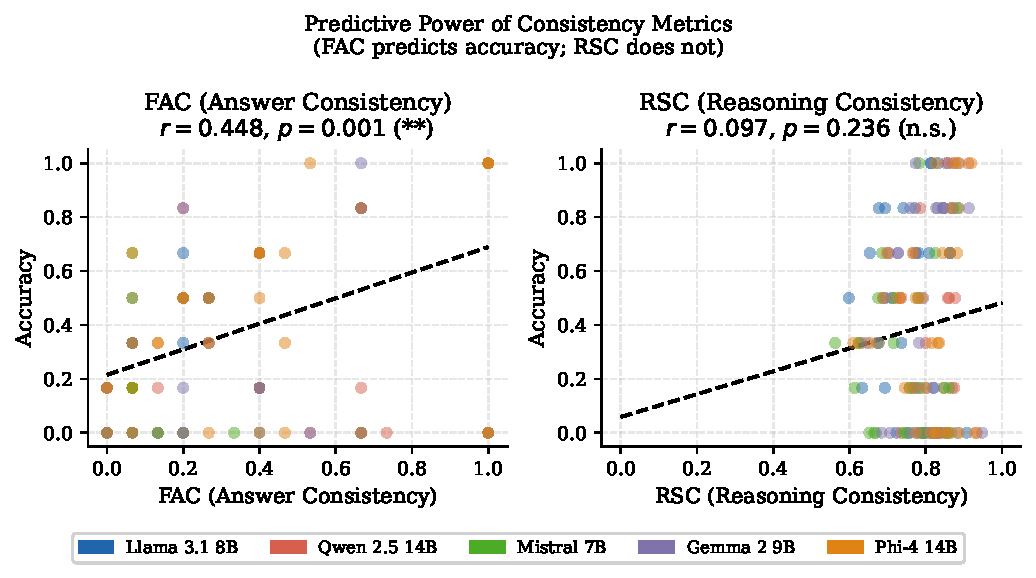
\includegraphics[width=0.8\linewidth]{../figures/fig4_fac_accuracy.pdf}
\caption{Scatter plots showing the relationship between consistency metrics and problem accuracy. FAC is a strong predictor of accuracy, while RSC shows almost no correlation.}
\label{fig:scatter}
\end{figure}

Final Answer Consistency (FAC) is a strong positive predictor of accuracy (Pearson $r = 0.448, p < 0.001$). Problems where the model consistently arrives at the same answer across paraphrases are highly likely to be answered correctly. This aligns with the foundational premise of Self-Consistency \citep{wang2023selfconsistencyimproveschainthought}.

Conversely, Reasoning Step Consistency (RSC) shows virtually no correlation with accuracy (Pearson $r = 0.097, p = 0.236$). A model can produce highly consistent reasoning chains across paraphrases and still be completely wrong. This is a critical finding for interpretability: the stability or coherence of a reasoning chain is not a reliable indicator of its correctness or its causal link to the correct answer.

\section{Discussion}

The universal negativity of the Answer-Reasoning Consistency Gap (ARCG) provides compelling evidence for what we term the ``execution gap'' in LLM reasoning. Under natural semantic variation, LLMs do not exhibit post-hoc rationalization; rather, they exhibit execution fragility.

When presented with a problem, an LLM reliably retrieves a relevant reasoning template from its training distribution. This template is robust to surface-level paraphrasing, resulting in high Reasoning Step Consistency (RSC). However, the model struggles to execute the specific logical or arithmetic operations required by that template to reach the correct conclusion for the specific phrasing of the prompt. A slight change in wording causes the final execution step to fail, resulting in low Final Answer Consistency (FAC).

This finding has significant implications for the interpretability of Chain-of-Thought. If a reasoning chain is highly stable but the final answer is fragile, the reasoning chain cannot be viewed as a strict causal derivation of the answer. Instead, the reasoning chain is a stable artifact of the prompt's general semantic neighborhood, while the final answer is a brittle product of the exact token sequence. Consequently, auditing an LLM's reasoning chain for correctness does not guarantee that the model will reliably produce the correct answer in deployment.

Furthermore, our results highlight a limitation of current consistency-based decoding methods. While majority voting over answers (Self-Consistency) improves performance by mitigating FAC fragility, it does not address the underlying execution gap. Future work should explore decoding strategies or training interventions that explicitly align the execution of reasoning steps with the final output generation.

\section{Conclusion}

We introduced the Answer-Reasoning Consistency Gap (ARCG) to quantify the decoupling between reasoning stability and answer stability in LLMs. Through systematic evaluation of five open-source models, we demonstrated that ARCG is universally negative: reasoning chains are significantly more robust to semantic paraphrasing than final answers. This finding challenges the post-hoc rationalization hypothesis and exposes an ``execution gap'' where models reliably retrieve reasoning templates but fail to execute them consistently. Our work underscores the need for new interpretability metrics that account for the fragile link between generated logic and final outcomes in large language models.

\section*{Acknowledgments}
The author acknowledges the use of Large Language Models (LLMs) in the preparation of this manuscript. Specifically, an LLM was utilized to generate the Python code for the experimental pipeline, produce the data visualization plots, and assist in drafting and refining the prose of this paper. The core research ideation, experimental design, and metric formulation (ARCG) were conducted independently by the human author. This disclosure is made in accordance with the COLM 2026 Policy on Large Language Model Usage.

\bibliography{references}
\bibliographystyle{colm2026_conference}

\end{document}
